\section{Définitions Fondamentales des Graphes}



\begin{figure}[H]
    \centering
    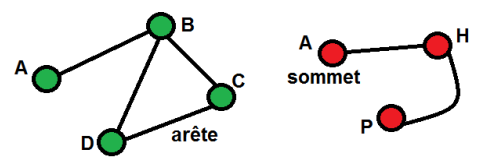
\includegraphics{Assets/graphes.PNG}
    \caption{Graphe , Sommet , Arete}
    \label{fig:enter-label}
\end{figure}
\subsection{Graphe}
Un graphe \( G \) est une paire ordonnée \( G = (V, E) \) où \( V \) est un ensemble de sommets et \( E \) est un ensemble d'arêtes reliant ces sommets. Les graphes sont utilisés pour modéliser des relations binaires entre des éléments.

\subsection{Sommets (ou Nœuds)}
Les sommets \( v \in V \), aussi appelés nœuds, sont les unités de base d'un graphe. Ils peuvent représenter divers objets selon le contexte, comme des individus dans un réseau social ou des intersections dans un réseau routier.

\subsection{Arêtes (ou Liens)}
Les arêtes \( e \in E \), ou liens, sont des paires de sommets qui indiquent une relation ou une connexion entre eux. Dans un graphe non orienté, l'arête \( (u, v) \) est identique à \( (v, u) \), signifiant une relation bidirectionnelle.



\subsection{Graphe non orienté}
Un graphe est dit non orienté si ses arêtes n'ont pas de direction spécifique, permettant un déplacement libre entre les sommets connectés.
\begin{figure}[H]
    \centering
    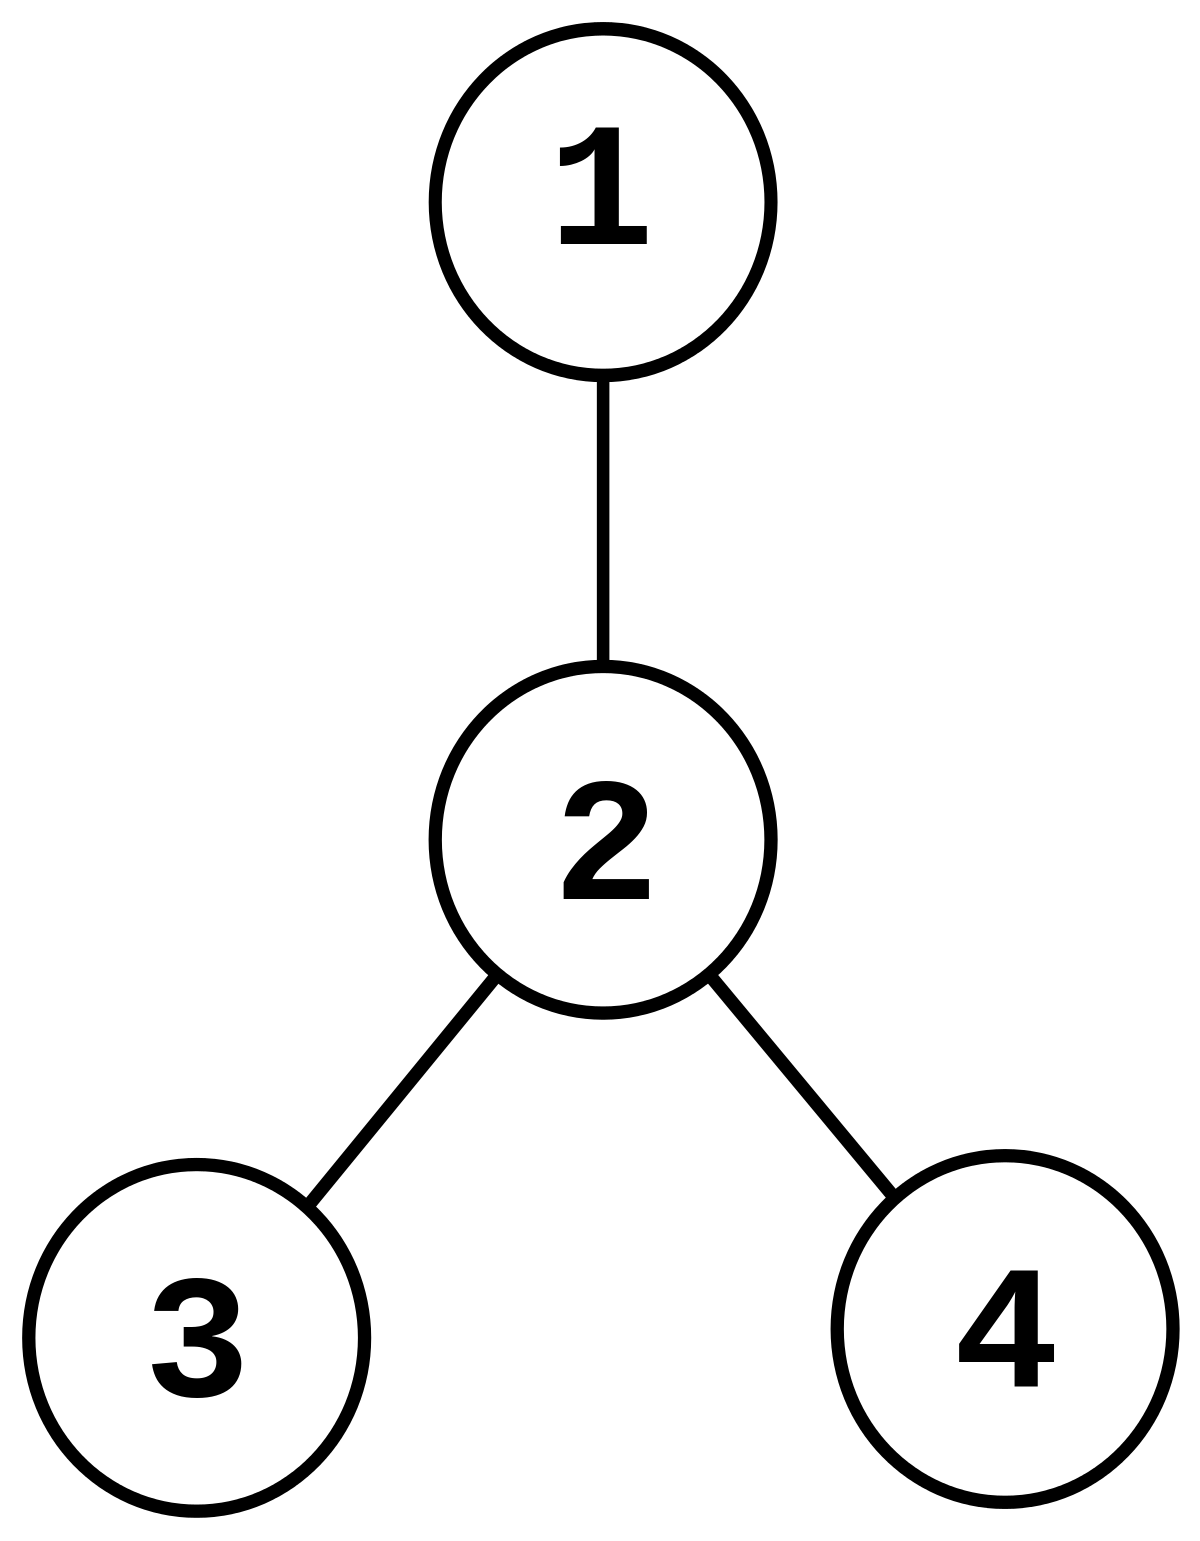
\includegraphics[width=0.3 \textwidth]{Assets/grapheNonOriente.png}
    \caption{Graphe non orienté}
    \label{fig:Graphe non orienté}
\end{figure}



\subsection{Graphe orienté (ou Digraphe)}
Un graphe orienté, ou digraphe, est un graphe où chaque arête \( (u, v) \) a une direction allant de \( u \) à \( v \), représentant une relation unidirectionnelle.

\begin{figure}[H]
    \centering
    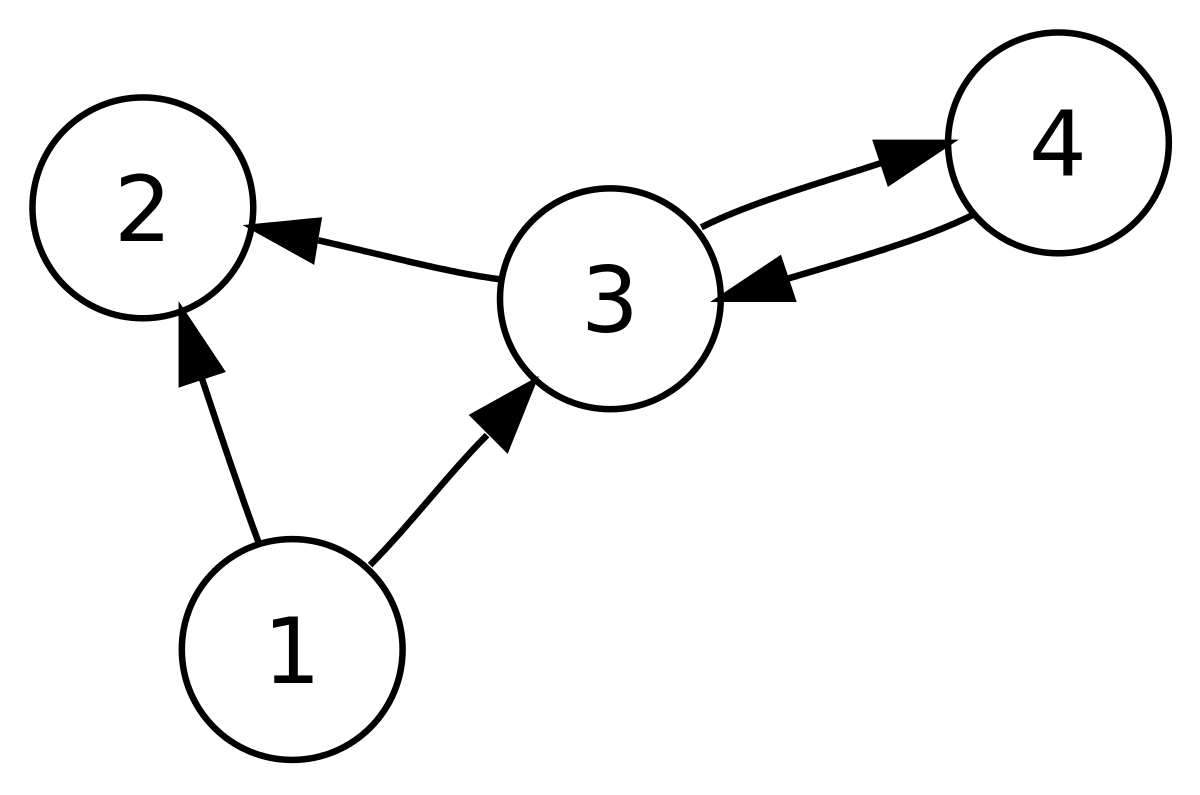
\includegraphics[width=0.4 \textwidth]{Assets/grapheOriente.png}
    \caption{Graphe orienté}
    \label{fig:Graphe orienté}
\end{figure}



\subsection{Graphe pondéré}
Un graphe pondéré est un graphe où chaque arête \( e \) se voit attribuer un poids \( w(e) \), qui peut représenter une mesure comme la distance, le coût, ou la capacité.
\begin{figure}[H]
    \centering
    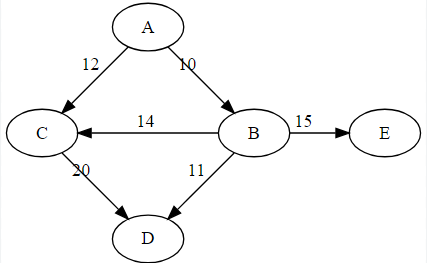
\includegraphics[width=0.4 \textwidth]{Assets/GraphePondere.PNG}
    \caption{Graphe pondéré}
    \label{fig:Graphe pondéré}
\end{figure}


\subsection{Graphe connexe}
Un graphe est connexe si pour tout couple de sommets \( u, v \in V \), il existe un chemin les reliant.

\begin{figure}[H]
    \centering
    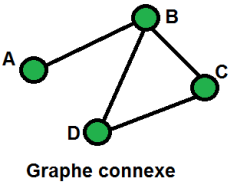
\includegraphics[width=0.3 \textwidth]{Assets/Graphe Connexe.PNG}
    \caption{Graphe Connexe }
    \label{fig:Graphe Connexe}
\end{figure}

%%%%%%%%%%%%%%%%%%%%%%%%



\newpage



%%%%%%%%%%%%%%%%%

\subsection{Graphe non connexe}
Un graphe est dit non connexe s'il existe au moins un couple de sommets \( u, v \in V \) entre lesquels aucun chemin n'existe. Cela signifie qu'il n'est pas possible de se rendre de \( u \) à \( v \) en suivant les arêtes du graphe. Un graphe non connexe peut être constitué de plusieurs composantes connexes isolées les unes des autres.

\begin{figure}[H]
    \centering
    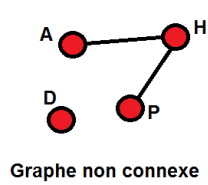
\includegraphics[width=0.3 \textwidth]{Assets/Graphe Non Connexe.PNG}
    \caption{Graphe Non Connexe }
    \label{fig:Graphe Non Connexe}
\end{figure}




\subsection{Cycle}
Un cycle est une séquence de sommets distincts commençant et se terminant par le même sommet, avec chaque paire de sommets consécutifs étant connectée par une arête.

\begin{figure}[H]
    \centering
    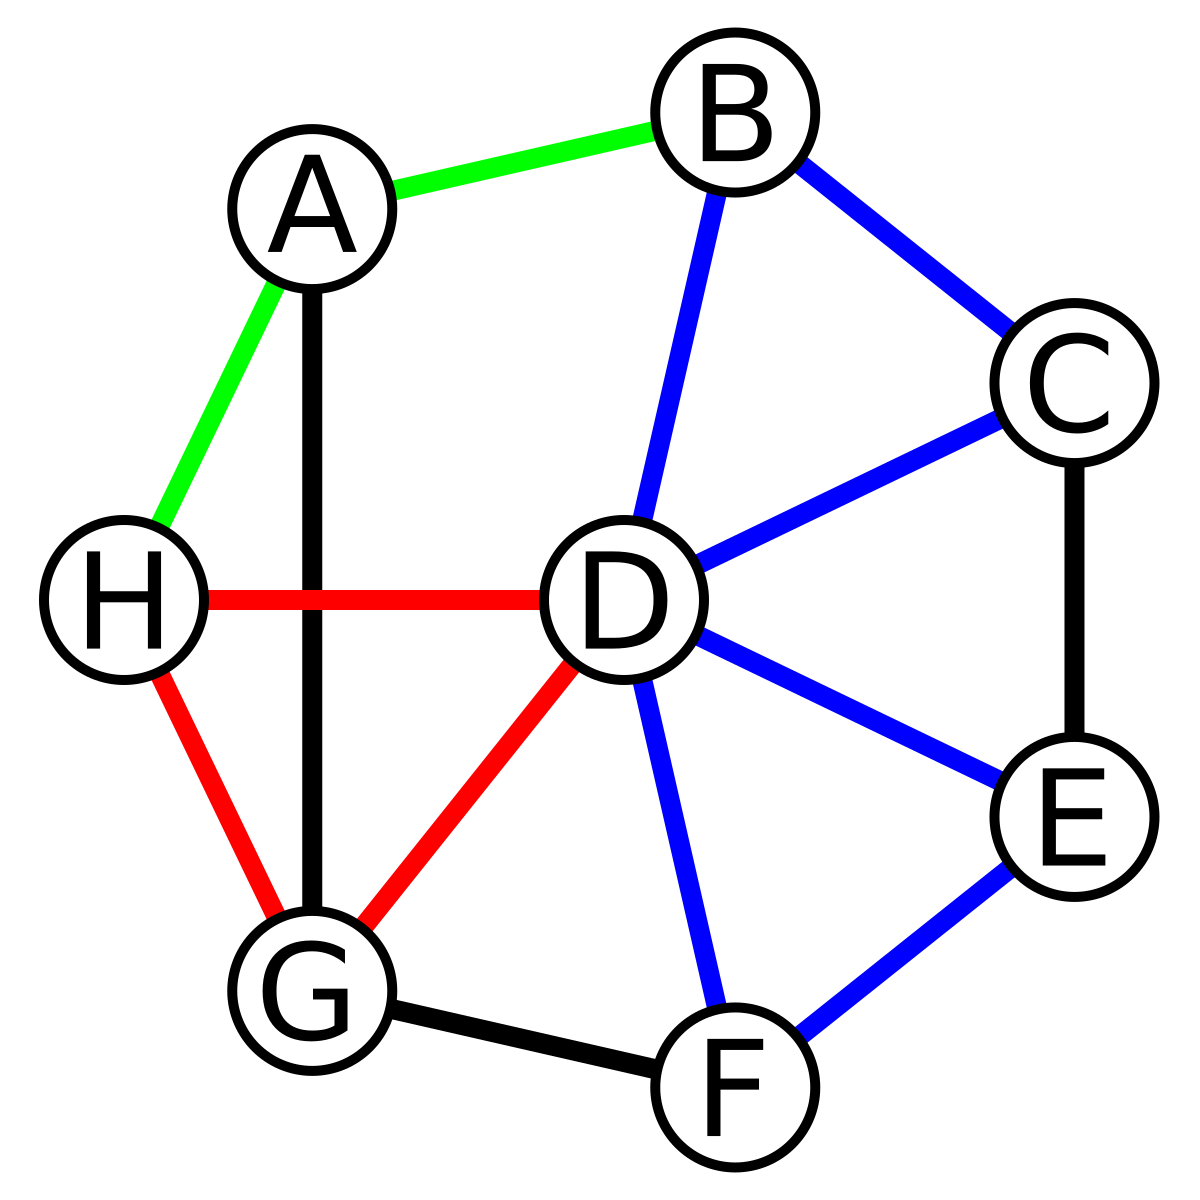
\includegraphics[width=0.5 \textwidth]{Assets/cycle.png}
    \caption{Cycle}
    \label{fig: Cycle}
\end{figure}



\subsection{Chemin}
Un chemin est une séquence de sommets où chaque paire de sommets consécutifs est reliée par une arête. Dans un graphe orienté, les arêtes du chemin doivent être suivies dans la direction spécifiée.

\begin{figure}[H]
    \centering
    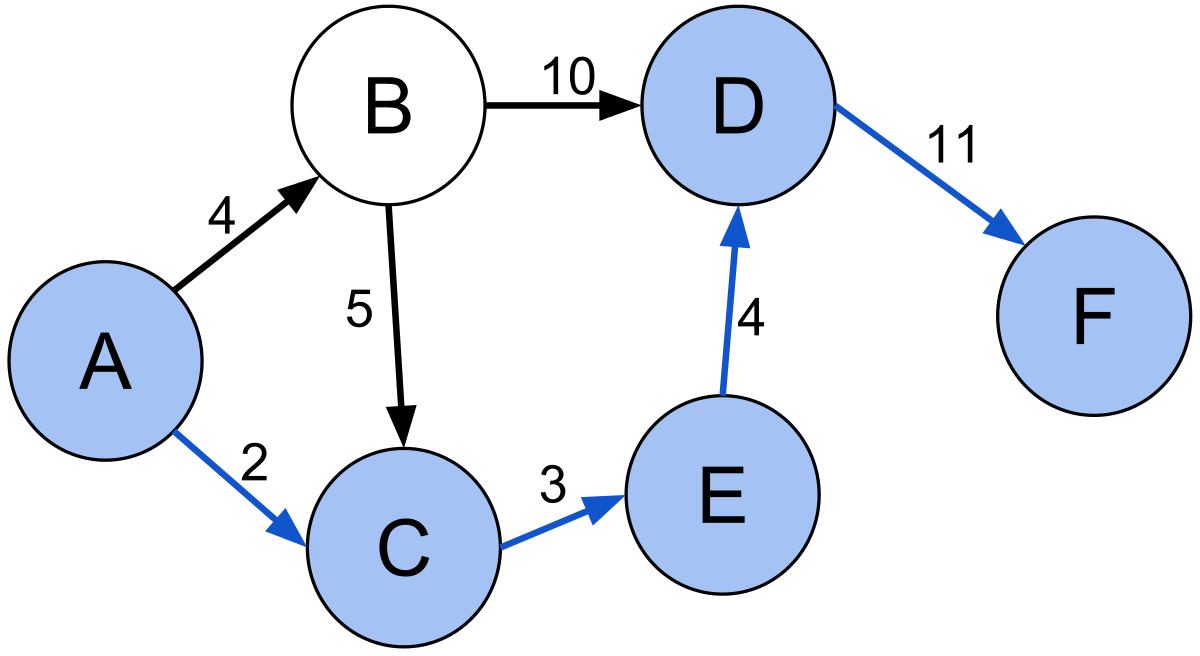
\includegraphics[width=0.5 \textwidth]{Assets/chemin.png}
    \caption{Chemin}
    \label{fig: Chemin}
\end{figure}